% Chapter 4
\chapter{SYSTEM DESIGN} % All Chapter headings in ALL CAPS

\section{Overall Architecture}
The goal of this project is to build a module that facilitates the necessary optimizations pertaining to predictive commoning. This entails a few key modules which are diagrammatically represented in Figure 4.1.
\newline

\begin{figure}[H]
	\centering
	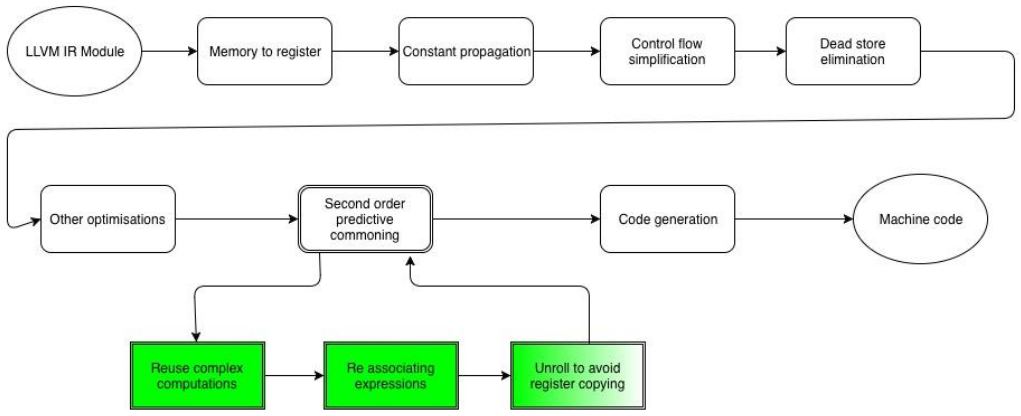
\includegraphics[scale=0.45]{block.png}
	\caption{Architecture Diagram}
	\label{ArchDia}	
\end{figure}


The first module deals with identifying what parts of the code will be targeted for the optimization. The LLVM API provides interfaces to identify and target code i.e.\ it helps to target only loops instead of running through the entire program. \\ 

This overall architecture can be decomposed into a few highly cohesive modules. Each module is explained in detail in the following section.

\section{Modules}
\subsection{Identifying computation expressions}

This module is responsible for identification of array indexing operations. It does this by connecting the multiple instructions that make up an indexing expression and grouping them as one basic block.

It repeats the process for all the instructions and returns a list of such expressions.

\begin{algorithm}
	\caption{Identifying indexed sequences}
	\begin{algorithmic}
		\STATE $V \leftarrow$ Empty vector
		\FOR{\textbf{each} $getElementPtrInst$}
		\STATE $dominantLoad \leftarrow findDominantLoad()$
		\STATE $dominatedLoad \leftarrow findDominatedLoad()$
		\IF {$dominantLoad \neq $ null AND $dominatedLoad \neq $ null}
		\STATE $V.push(indexed expressions)$
		\ENDIF
		\ENDFOR
		\RETURN $V$
	\end{algorithmic}
\end{algorithm}


\subsection{Annotate Computation Expressions}

Once we have identified the necessary expressions, we then annotate them with useful meta data. It is one of the ways through which information is sent across passes. We use this to tag two pieces of meta data, namely

\begin{itemize}
	\item Type of indexed expression
	\item Initial value of an indexed expression
\end{itemize}


\begin{algorithm}
	\caption{Initial value calculation}
	\begin{algorithmic}
		
		\FOR{\textbf{each} $GEPInstruction$}
		\STATE $dominantLoad \leftarrow findDominantLoad()$
		
		\FOR{\textbf{each} instruction \textbf{between} $dominantLoad$ AND $GEPInstruction$}
		\IF {\textbf{type of}instruction $==$ arithmetic Op}
		\IF {operand $==$ constant}
		\RETURN constant
		\ENDIF
		\ENDIF
		\RETURN 0
		\ENDFOR
		\ENDFOR
		
	\end{algorithmic}
\end{algorithm}

\begin{algorithm}
	\caption{Annotate computation expressions}
	\begin{algorithmic}
		
		\STATE \textbf{Input:} Vector of indexed expressions $V$
		
		\FOR{\textbf{each} indexed expression \textbf{in} $V$}
		\STATE $node \leftarrow getSuccessor()$
		
		\IF {\textbf{typeof} node $==$ load}
		\STATE Tag as LHS
		\STATE $initialValue \leftarrow getIntialValue()$
		\STATE Tag initialValue to indexed expression
		\ENDIF
		\ENDFOR
		\RETURN V
		
	\end{algorithmic}
\end{algorithm}

\subsection{Reassociate Expressions}

The optimization work begins with this phase. We hoist the LHS indexed expressions out of the loop into new registers. After hoisting, these are then initialized with the value retrieved from the meta data attached earlier. We then proceed to add re-associating  expressions i.e\ the swap instructions between the registers. 
\\

\begin{algorithm}
	\caption{Re-associating expressions}
	\begin{algorithmic}
		\STATE \textbf{Input:} Vector of tagged indexed expressions $V$
		\STATE Create a BasicBlock above the loop header
		\FOR{\textbf{each} RHS indexed expression}
		\STATE Create a register in the hoisted block
		\STATE Get initial value of indexed expression from meta data
		\STATE Load value into register
		\ENDFOR
		
	\end{algorithmic}
\end{algorithm}

\newpage
\subsection{Remove Dead Instructions}

Once all the optimizations are done, we need to find and eliminate all instructions which are now deemed unnecessary. Here, we make use LLVM's advanced Uses and Users APIs to complete the task. \\

\begin{algorithm}
	\caption{Re-associating expressions}
	\begin{algorithmic}
		\FOR{\textbf{each} instruction \textbf{in} BasicBlock}
		\STATE $users \leftarrow getAllUsers(instruction) $
		\IF {users \textbf{is} empty}
		\STATE $removeInstruction(instruction)$
		\STATE $replaceAllUsesWith(undefinedValue)$
		\ENDIF
		\ENDFOR
	\end{algorithmic}
\end{algorithm}